%%chang the compiler to Xelatex
\documentclass{article}%%attention!!!!!!!!!!!!!!!!!!!!!!!!!!!
\usepackage{enumerate,float,bbding,booktabs,diagbox,graphicx,tabularx,subfigure,amsmath,listings,color,multicol,multirow,wrapfig,calligra,tikz,tcolorbox,geometry,hyperref,xcolor,url,underscore}
\usepackage[fontset=ubuntu]{ctex}%%attention !!!!!!!!!!!!!!!!!!!!!!!!!!!!
% xcolor-高亮使用的颜色
 \geometry{a4paper,scale=0.85}
\definecolor{dkgreen}{rgb}{0,0.6,0}
\definecolor{gray}{rgb}{0.5,0.5,0.5}
\definecolor{mauve}{rgb}{0.58,0,0.82}
\lstset{
  basicstyle=\tt,
  frame=tb,
  language=C++,
  aboveskip=3mm,
  belowskip=3mm,
  showstringspaces=false,
  columns=flexible,
  basicstyle={\small\ttfamily},
  numbers=left,%设置行号位置none不显示行号
  %numberstyle=\tiny\courier, %设置行号大小  
  numberstyle=\tiny\color{gray},
  keywordstyle=\color{blue},
  commentstyle=\color{dkgreen},
  stringstyle=\color{mauve},
  breaklines=true,
  breakatwhitespace=true,
  escapeinside=``,%逃逸字符(1左面的键),用于显示中文例如在代码中`中文...`
  tabsize=4,
  extendedchars=false %解决代码跨页时,章节标题,页眉等汉字不显示的问题  
}
\usetikzlibrary{mindmap}% 画思维导图用
\begin{document}
\begin{titlepage}
     \begin{center}
          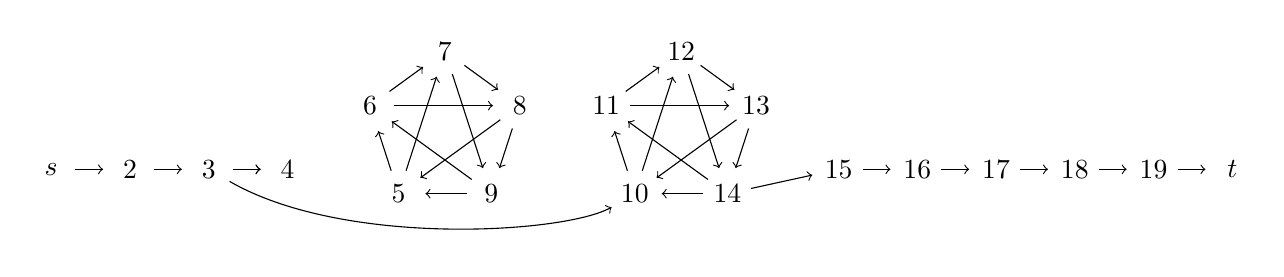
\begin{tikzpicture}[shorten >=1pt,->]
               \tikzstyle{vertex}=[circle,fill=white!25,minimum size=17pt,inner sep=0pt]
               \foreach \name/\x in {s/1, 2/2, 3/3, 4/4, 15/11, 
                                     16/12, 17/13, 18/14, 19/15, t/16}
                 \node[vertex] (G-\name) at (\x,0) {$\name$};
             
               \foreach \name/\angle/\text in {P-1/234/5, P-2/162/6, 
                                               P-3/90/7, P-4/18/8, P-5/-54/9}
                 \node[vertex,xshift=6cm,yshift=.5cm] (\name) at (\angle:1cm) {$\text$};
             
               \foreach \name/\angle/\text in {Q-1/234/10, Q-2/162/11, 
                                               Q-3/90/12, Q-4/18/13, Q-5/-54/14}
                 \node[vertex,xshift=9cm,yshift=.5cm] (\name) at (\angle:1cm) {$\text$};
             
               \foreach \from/\to in {s/2,2/3,3/4,3/4,15/16,16/17,17/18,18/19,19/t}
                 \draw (G-\from) -- (G-\to);
             
               \foreach \from/\to in {1/2,2/3,3/4,4/5,5/1,1/3,2/4,3/5,4/1,5/2}
                 { \draw (P-\from) -- (P-\to); \draw (Q-\from) -- (Q-\to); }
             
               \draw (G-3) .. controls +(-30:2cm) and +(-150:1cm) .. (Q-1);
               \draw (Q-5) -- (G-15);
             \end{tikzpicture}

             \vspace{100pt}

     \Huge{C++}
    \vspace{250pt}

    \large{11180708 忻宇}
     \end{center}
\end{titlepage}
\tableofcontents
 
\section{Function Review}
Return:
\begin{enumerate}
    \item return type
    \begin{enumerate}
        \item C++ does place a restriction on what types you can use for a return value:The return value cannot be an array.Everything else is possible—integers,floating-point numbers,pointers,and even structures and objects!
       \item Interestingly,even though a C++ function can’t return an array directly,it can return an array that’s part of a structure or object.
    \end{enumerate}
    \item return process
     \begin{enumerate}
         \item a function returns a value by copying the return value to a specified CPU register or memory location
         \item Then the calling program examines that location
     \end{enumerate}
\end{enumerate}
应嘉之
\end{document}
